In diesem Versuch geht es darum mithilfe eines Laserentfernungsmessers die Brechzahl von zwei transparenten, nicht-diffusen Materialien zu bestimmen. Das ist möglich, da der Laserentfernungsmesser, die Lichtgeschwindigkeit als konstant annimmt. Dadurch zeigt das Gerät eine größere Distanz an, als es tatsächlich der Fall ist, mit dieser Tatsache lässt sich nun die Brechzahl bestimmen. Für die Brechzahlen gilt folgender Zusammenhang:

\begin{equation}
    n = \frac{c_{Vakuum}}{c_{Material}}
\end{equation}

Wir nehmen in diesem Versuch der Einfachheit halber an, dass gilt:

\begin{equation}
    n_{Luft} = 1.000272 \approx 1 = n_{Vakuum} \Rightarrow n_{Luft} \approx n_{Vakuum}
\end{equation}

Der Versuchsaufbau ist in Abbildung \ref{fig:Laserentfernungsmesser} skizziert. Die Ergebnisse der Messungen sind in Tabelle \ref{tab:Messwerte Versuch 3 Lichtgeschwindigkeit} aufgetragen.

\begin{figure}[h]
    \centering
    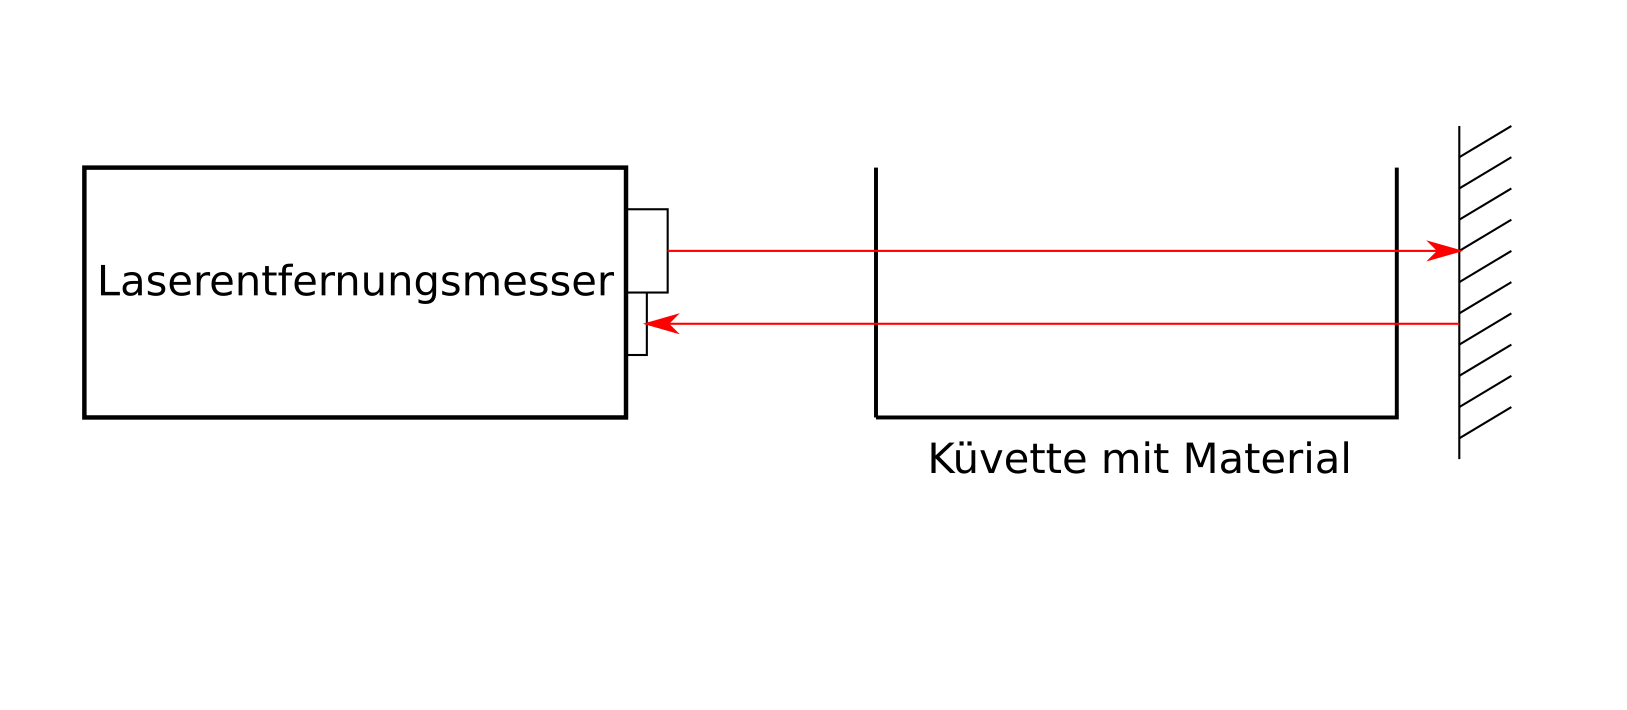
\includegraphics[scale=0.6]{./fig/Laserentfernungsmesser.png}
    \caption{Versuchaufbau für die Brechzahlbestimmung mit modernem Laserentfernungsmesser}
    \label{fig:Laserentfernungsmesser}
\end{figure}

\begin{table}
    \centering
    \caption{Messwerte für die Brechzahlbestimmung mit modernem Laserentfernungsmesser (Mittelwerte)}
    \begin{tabular}{c c c}
    \hline
    Material & Abstand in mm (quer) & Abstand in mm (längs) \\
    \hline
    Nichts & 351 & 351 \\
    Leere Küvette & - & 358.75 \\
    Silikonöl & 377 & 396.25 \\
    Wasser & 374.25 & 390.25 \\
    \hline
    \end{tabular}
    \label{tab:Messwerte Versuch 3 Lichtgeschwindigkeit}
\end{table}

Es gilt allgemein:

\begin{equation}
    t_i = \frac{s_i}{c_i} 
\end{equation}

Die Indizes geben dabei das Material an und "0" \, für die Messung mit leerer und "Gerät" \, für die Messung mit Material in der Küvette. Es folgt für die Zeit für die leere Küvette:

\begin{equation} \label{Gleichung t leer}
    t_{0} = \frac{s_{Luft} - s_{Glas}}{c_{Luft}} + \frac{s_{Glas}}{c_{Glas}} = \frac{s_{Luft}}{c_{Luft}} - \frac{s_{Glas}}{c_{Luft}} + \frac{s_{Glas}}{c_{Glas}}
\end{equation}

Daraus folgt für die Zeit für die Küvette mit Material: 

\begin{equation} \label{Gleichung t Mat}
    t_{\text{Gerät}} = \frac{s_{Luft} -s_{Glas} -s_{Mat}}{c_{Luft}} + \frac{s_{Glas}}{c_{Glas}} + \frac{s_{Luft}}{c_{Luft}} = \frac{s_{Luft}}{c_{Luft}} - \frac{s_{Glas}}{c_{Luft}} - \frac{s_{Mat}}{c_{Luft}} + \frac{s_{Glas}}{c_{Glas}} + \frac{s_{Mat}}{c_{Mat}}
\end{equation}

Damit folgt für die Differenz aus Gleichung \ref{Gleichung t leer} und \ref{Gleichung t Mat}

\begin{equation}
    t_{\text{Gerät}} - t_{0} = \frac{s_{Mat}}{c_{Mat}} - \frac{s_{Mat}}{c_{Luft}} = \frac{s_{\text{Gerät}}}{c_{\text{Gerät}}} - \frac{s_0}{s_0}
\end{equation}

Daraus folgt:

\begin{align}
    s_{\text{Gerät}} - s_0 &= s_{Mat} (\frac{c_{Luft}}{c_{Mat}} - 1) \\
    \Rightarrow n &= \frac{c_{Luft}}{c_{Mat}} = \frac{s_{\text{Gerät}} - s_0}{s_{Mat}} + 1
\end{align}

Es folgt durch einsetzen für die Brechzahlen von Wasser und Silikonöl:

\begin{table}[h]
    \caption{Brechzahlen ermittelt mit modernem Laserentfernungsmesser}
    \label{tab:Brechzahlen Laser}
    \centering
    \begin{tabular}{c c c c c}
    \hline
    Material & Brechzahl (quer) & Brechzahl (längs) & Mittelwert & Literaturwert\\
    \hline
    Silikonöl & 1.365 & 1.375 & 1.370 & 1.4 \\
    Wasser & 1.310 & 1.315 & 1.313 & 1.33 \\
    \hline
    \end{tabular}
    Quelle Literaturwerte: \url{https://www.microscope.healthcare.nikon.com/de_EU/products/optics/silicone-immersion-series}
\end{table}

 Wie man an den erhaltenen Werte gut erkennen kann, sind diese für das gewählte Messverfahren relativ genau. Für die Brechzahl von Silikonöl erhalten wir eine Abweichung von nur ca. 3\% und für die Brechzahl von Wasser von nur ca. 1\% zum Literaturwert. Was auch an den Werten zu erkennen ist, ist, dass der Wert für die Messung mit längs zum Laser orientierten Kürvette näher am Literaturwert liegt. Was daran liegt, dass die Strecke, die das Licht tatsächlich durch das Material geht größer ist, was zu einem genaueren Wert führt.
 
 Mögliche Fehlerquellen sind: 
 
 \begin{itemize}
     \item Eichung des Laserentfernungsmesser
     \item Genauigkeit des Laserentfernungsmesser (Genauigkeit $\pm \SI{1.5}{\milli\metre}$)
     \item Reflexion an der Glaswand der Küvette
     \item Verschmutzungen an der Wand der Küvette oder im Material
 \end{itemize}
 
 Angesichts der Messmethode und deren Ungenauigkeit ist das Ergebnis aber zufriedenstellend.